\documentclass[11pt]{article}
\usepackage{amsmath, amssymb, mathtools, bm}
\usepackage{physics}
\usepackage{tikz}
\usetikzlibrary{decorations.pathmorphing,arrows.meta,calc,positioning}
\usepackage[margin=2.3cm]{geometry}
\usepackage{siunitx}
\usepackage{booktabs}
\usepackage{hyperref}
\usepackage{braket}

\newcommand{\de}{\mathrm{d}}

\title{B3: Quantum, Atomic \& Molecular Physics --- Model Solutions, Trinity 2019}
\author{}
\date{}

\begin{document}
\maketitle

%==================================================================
\section*{Question 1 --- LS coupling, fine structure, Mg \& Ba}
%==================================================================

\subsection*{(a) The LS-coupling scheme}

\textbf{Problem.} \emph{Explain what is meant by the LS-coupling scheme. Outline how the residual electrostatic interaction leads to the formation of terms, and explain why these can be labelled by $L$ and $S$.}

LS coupling applies when the residual electrostatic (electron--electron) interaction $H_{\rm ee}$ greatly exceeds the spin--orbit interaction $H_{\rm SO}$. Treat $H_{\rm ee}$ first, $H_{\rm SO}$ as a perturbation on top.

The unperturbed central-field Hamiltonian commutes with each $\bm l_i$ and $\bm s_i$. The residual electrostatic interaction
\[
H_{\rm ee}=\sum_{i<j}\frac{e^{2}}{4\pi\epsilon_0 r_{ij}}-\sum_i V_{\rm cf}(r_i)
\]
is spin-independent and rotationally invariant: it commutes with $\bm L=\sum_i\bm l_i$ and $\bm S=\sum_i\bm s_i$.

Hence $L^{2},L_z,S^{2},S_z$ remain good quantum numbers; eigenstates within a configuration split into \emph{terms} $^{2S+1}L$, each $(2L+1)(2S+1)$-fold degenerate.

\subsection*{(b) Spin--orbit interaction and the interval rule}

\textbf{Problem.} \emph{Explain how the spin--orbit interaction leads to fine structure in LS coupling, and derive the interval rule.}

Within a term, $H_{\rm SO}=\sum_i\xi(r_i)\,\bm l_i\!\cdot\!\bm s_i$. Project onto the term using the projection theorem (Land\'e):
\[
H_{\rm SO}\big|_{^{2S+1}L}=\beta(L,S)\,\bm L\!\cdot\!\bm S.
\]
Couple $\bm J=\bm L+\bm S$:
\[
\bm L\!\cdot\!\bm S=\tfrac12\bigl(\bm J^{2}-\bm L^{2}-\bm S^{2}\bigr).
\]
Take the diagonal element in $\ket{LSJ}$:
\[
\Braket{\bm L\!\cdot\!\bm S}_J=\tfrac{\hbar^{2}}{2}\bigl[J(J+1)-L(L+1)-S(S+1)\bigr].
\]
Fine-structure level energy:
\[
E_J=E_0+\tfrac{\beta\hbar^{2}}{2}\bigl[J(J+1)-L(L+1)-S(S+1)\bigr].
\]
Splitting between adjacent levels $J$ and $J-1$:
\[
E_J-E_{J-1}=\tfrac{\beta\hbar^{2}}{2}\bigl[J(J+1)-(J-1)J\bigr].
\]
Simplify $J(J+1)-(J-1)J=2J$:
\begin{equation}
\boxed{\;E_J-E_{J-1}=\beta\hbar^{2}\,J.\;}
\label{eq:interval}
\end{equation}
The splitting is proportional to the larger $J$: this is Land\'e's interval rule.

\subsection*{(c) Mg energy-level diagram}

\textbf{Problem.} \emph{Use the listed Mg lines and the 3s4s singlet--triplet splitting to construct the energy-level diagram, identify the transitions, give level energies in $\unit{m^{-1}}$, and test the interval rule.}

Three lowest configurations of Mg: $3s^{2}$, $3s3p$, $3s4s$, giving terms
\[
3s^{2}\;{}^{1}\!S_0,\qquad 3s3p\;{}^{1}\!P_1,\,{}^{3}\!P_{0,1,2},\qquad 3s4s\;{}^{1}\!S_0,\,{}^{3}\!S_1.
\]
Convert each wavelength to wavenumber $\tilde\nu=1/\lambda$:
\begin{align*}
\lambda=\SI{285.21}{nm}&:\;\tilde\nu=3.50621\times 10^{6}\ \unit{m^{-1}},\\
\lambda=\SI{516.73}{nm}&:\;\tilde\nu=1.93525\times 10^{6}\ \unit{m^{-1}},\\
\lambda=\SI{517.27}{nm}&:\;\tilde\nu=1.93323\times 10^{6}\ \unit{m^{-1}},\\
\lambda=\SI{518.36}{nm}&:\;\tilde\nu=1.92917\times 10^{6}\ \unit{m^{-1}},\\
\lambda=\SI{1182.8}{nm}&:\;\tilde\nu=8.45452\times 10^{5}\ \unit{m^{-1}}.
\end{align*}

Identify lines using E1 selection rules ($\Delta S=0$, $\Delta L=0,\pm1$, $\Delta J=0,\pm1$):

\textbf{285.21\,nm (absorption from ground).} Only allowed E1 line ex $3s^{2}\,{}^{1}\!S_0$ is to $3s3p\,{}^{1}\!P_1$:
\[
E({}^{1}\!P_1)=3.50621\times 10^{6}\ \unit{m^{-1}}.
\]

\textbf{1182.8\,nm.} Singlet line $3s4s\,{}^{1}\!S_0\to 3s3p\,{}^{1}\!P_1$:
\[
E(3s4s\,{}^{1}\!S_0)=3.50621\times 10^{6}+8.45452\times 10^{5}=4.35166\times 10^{6}\ \unit{m^{-1}}.
\]

Use given singlet--triplet splitting $\SI{230590}{m^{-1}}$:
\[
E(3s4s\,{}^{3}\!S_1)=4.35166\times 10^{6}-2.30590\times 10^{5}=4.12107\times 10^{6}\ \unit{m^{-1}}.
\]

\textbf{Triplet lines: $3s4s\,{}^{3}\!S_1\to 3s3p\,{}^{3}\!P_{J}$.} Higher photon energy reaches lower-energy $^{3}\!P_J$ (normal ordering $J=0<1<2$):
\begin{align*}
E({}^{3}\!P_0)&=4.12107\times 10^{6}-1.93525\times 10^{6}=2.18582\times 10^{6}\ \unit{m^{-1}},\\
E({}^{3}\!P_1)&=4.12107\times 10^{6}-1.93323\times 10^{6}=2.18784\times 10^{6}\ \unit{m^{-1}},\\
E({}^{3}\!P_2)&=4.12107\times 10^{6}-1.92917\times 10^{6}=2.19190\times 10^{6}\ \unit{m^{-1}}.
\end{align*}

\paragraph{Interval-rule test.}
\[
E({}^{3}\!P_2)-E({}^{3}\!P_1)=4.06\times 10^{3}\ \unit{m^{-1}}.
\]
\[
E({}^{3}\!P_1)-E({}^{3}\!P_0)=2.02\times 10^{3}\ \unit{m^{-1}}.
\]
Ratio:
\[
\frac{E({}^{3}\!P_2)-E({}^{3}\!P_1)}{E({}^{3}\!P_1)-E({}^{3}\!P_0)}=2.01\approx 2.
\]
Land\'e \eqref{eq:interval} predicts $2:1$. \boxed{\text{Interval rule obeyed.}}

\paragraph{Energy-level diagram.}
\begin{center}
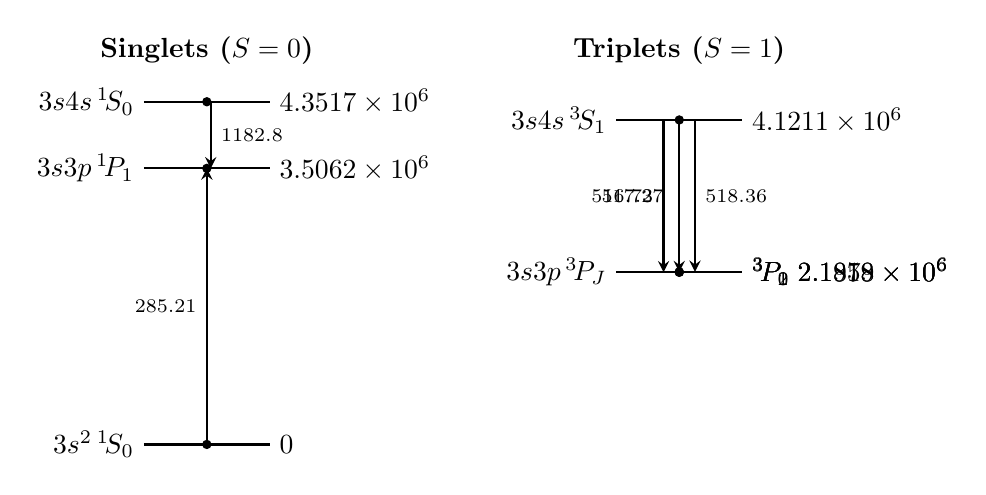
\begin{tikzpicture}[>=stealth, scale=1.0]
  % singlet column (left), triplet column (right)
  \def\xS{0}
  \def\xT{6}
  % vertical scale: 1 unit = 1e6 m^-1
  % ground
  \draw[thick] (\xS-0.8,0) -- (\xS+0.8,0);
  \node[left] at (\xS-0.8,0) {$3s^{2}\,{}^{1}\!S_{0}$};
  \node[right] at (\xS+0.8,0) {$0$};
  % 3s3p 1P1
  \draw[thick] (\xS-0.8,3.506) -- (\xS+0.8,3.506);
  \node[left] at (\xS-0.8,3.506) {$3s3p\,{}^{1}\!P_{1}$};
  \node[right] at (\xS+0.8,3.506) {$3.5062\times 10^{6}$};
  % 3s4s 1S0
  \draw[thick] (\xS-0.8,4.352) -- (\xS+0.8,4.352);
  \node[left] at (\xS-0.8,4.352) {$3s4s\,{}^{1}\!S_{0}$};
  \node[right] at (\xS+0.8,4.352) {$4.3517\times 10^{6}$};
  % 3s3p 3P012 (drawn as one cluster, expanded)
  \draw[thick] (\xT-0.8,2.186) -- (\xT+0.8,2.186);
  \node[right] at (\xT+0.8,2.186) {${}^{3}\!P_{0}\;2.1858\times 10^{6}$};
  \draw[thick] (\xT-0.8,2.188) -- (\xT+0.8,2.188);
  \node[right] at (\xT+0.8,2.188) {${}^{3}\!P_{1}\;2.1878\times 10^{6}$};
  \draw[thick] (\xT-0.8,2.192) -- (\xT+0.8,2.192);
  \node[right] at (\xT+0.8,2.192) {${}^{3}\!P_{2}\;2.1919\times 10^{6}$};
  \node[left] at (\xT-0.8,2.19) {$3s3p\,{}^{3}\!P_J$};
  % 3s4s 3S1
  \draw[thick] (\xT-0.8,4.121) -- (\xT+0.8,4.121);
  \node[left] at (\xT-0.8,4.121) {$3s4s\,{}^{3}\!S_{1}$};
  \node[right] at (\xT+0.8,4.121) {$4.1211\times 10^{6}$};
  % transitions
  \draw[->,thick] (\xS,0) -- (\xS,3.506) node[midway,left] {\scriptsize $285.21$};
  \draw[->,thick] (\xS+0.05,4.352) -- (\xS+0.05,3.506) node[midway,right] {\scriptsize $1182.8$};
  \draw[->,thick] (\xT-0.2,4.121) -- (\xT-0.2,2.186) node[midway,left] {\scriptsize $516.73$};
  \draw[->,thick] (\xT,4.121) -- (\xT,2.188) node[midway,left=2pt] {\scriptsize $517.27$};
  \draw[->,thick] (\xT+0.2,4.121) -- (\xT+0.2,2.192) node[midway,right] {\scriptsize $518.36$};
  % markers
  \node[circle,fill,inner sep=1.2pt] at (\xS,0) {};
  \node[circle,fill,inner sep=1.2pt] at (\xS,3.506) {};
  \node[circle,fill,inner sep=1.2pt] at (\xS,4.352) {};
  \node[circle,fill,inner sep=1.2pt] at (\xT,4.121) {};
  \node[circle,fill,inner sep=1.2pt] at (\xT,2.186) {};
  \node[circle,fill,inner sep=1.2pt] at (\xT,2.188) {};
  \node[circle,fill,inner sep=1.2pt] at (\xT,2.192) {};
  % labels for columns
  \node at (\xS,5.0) {\textbf{Singlets ($S=0$)}};
  \node at (\xT,5.0) {\textbf{Triplets ($S=1$)}};
\end{tikzpicture}
\end{center}

\subsection*{(d) Ba: validity of LS coupling}

\textbf{Problem.} \emph{Comment on whether LS coupling is a good approximation for Ba.}

LS-coupling expectation: each of $6s5d$ and $6s6p$ produces a singlet ($J=L$) plus a triplet $^{3}\!L_{L-1,L,L+1}$ obeying the interval rule (ratio $L+1:L$).

$6s6p$: triplet--triplet differences (\unit{m^{-1}}):
\[
1\,263\,662-1\,226\,602=37\,060.
\]
\[
1\,351\,474-1\,263\,662=87\,812.
\]
LS prediction $\Delta_{2,1}/\Delta_{1,0}=2$ requires ratio $2$:
\[
87\,812/37\,060=2.37.
\]
Singlet ${}^{1}\!P_1$ identified at $1\,806\,026\ \unit{m^{-1}}$ (well separated). Modest deviation from $2$ shows fine-structure perturbed by spin--orbit becoming comparable to triplet exchange splitting; LS \emph{still useful but breaking down}.

$6s5d$: differences:
\[
921\,550-903\,397=18\,153,\quad 959\,653-921\,550=38\,103.
\]
LS prediction $\Delta_{3,2}/\Delta_{2,1}=3/2=1.5$:
\[
38\,103/18\,153=2.10.
\]
Highest level $1\,139\,535$ assigned to $^{1}\!D_2$. Strong deviation from $1.5$, and $^{1}\!D_2$ lies anomalously close to the triplet (singlet--triplet $\sim 2\times 10^{5}\ \unit{m^{-1}}$, comparable to triplet width $\sim 2.4\times 10^{5}$). Term mixing significant.

\boxed{\text{LS coupling is only a rough approximation in Ba; intermediate coupling is required.}}

%==================================================================
\section*{Question 2 --- X-rays and Auger emission in Ag}
%==================================================================

\subsection*{(a) X-ray emission spectrum}

\textbf{Problem.} \emph{Processes responsible for X-ray emission under electron bombardment; describe the spectrum and its variation with $E_e$.}

Two processes:
\begin{enumerate}
\item \textbf{Bremsstrahlung}: deceleration of beam electrons in the Coulomb field of target nuclei produces a continuous spectrum extending to the Duane--Hunt cut-off $h\nu_{\max}=E_e$.
\item \textbf{Characteristic emission}: beam electrons knock out an inner-shell electron; an outer-shell electron radiatively fills the hole, emitting a photon at the energy difference of the two levels.
\end{enumerate}

As $E_e$ increases the bremsstrahlung end-point shifts to higher energy, and additional sets of characteristic lines (K, L, M, \ldots) appear once $E_e$ exceeds the corresponding shell binding energy.

\subsection*{(b) X-ray absorption spectrum}

\textbf{Problem.} \emph{Describe the absorption spectrum vs.\ $E_\gamma$ and link it to emission.}

Absorption follows a smooth $\sim E_\gamma^{-3}$ decrease, interrupted by sharp \emph{absorption edges} when $E_\gamma$ first exceeds an inner-shell binding energy ($K$, $L_1$, $L_2$, $L_3$, \ldots). Each edge marks the threshold for photo-ionising the corresponding shell; above the edge a new ionisation channel opens.

\paragraph{Linkage.}
\begin{itemize}
\item Each absorption edge sits at the binding energy of the hole-state initial level.
\item Characteristic emission lines lie at differences of binding energies, hence \emph{below} the absorption edge of the upper shell. E.g.\ $K$-edge $> $ all $K\alpha,K\beta$ emission lines.
\end{itemize}

\begin{center}
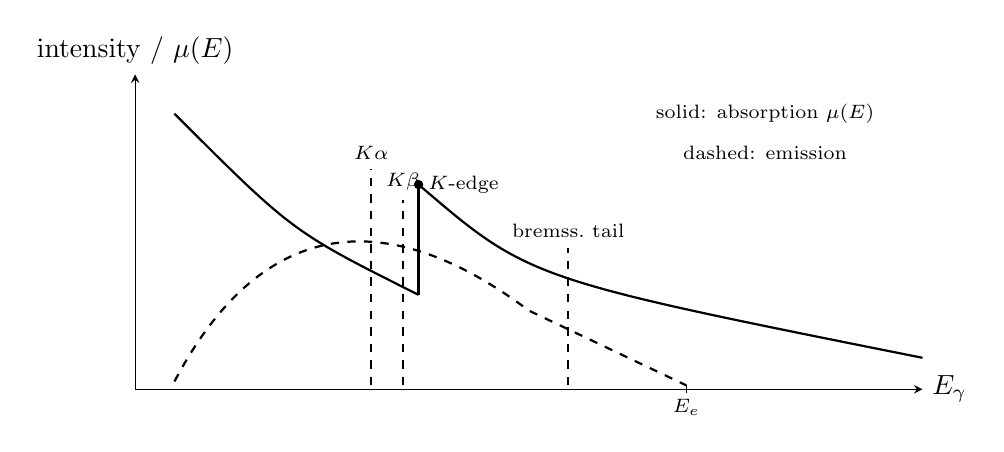
\begin{tikzpicture}[>=stealth, scale=1.0]
  \draw[->] (0,0) -- (10,0) node[right] {$E_\gamma$};
  \draw[->] (0,0) -- (0,4) node[above] {intensity / $\mu(E)$};
  % emission spectrum (lower curve, dashed)
  \draw[dashed,thick] (0.5,0.1) .. controls (1.5,2) and (3,2.5) .. (5,1.0) -- (7,0.05);
  \draw[dashed,thick] (3.0,0.05) -- (3.0,2.8);
  \draw[dashed,thick] (3.4,0.05) -- (3.4,2.4);
  \draw[dashed,thick] (5.5,0.05) -- (5.5,1.8);
  \node[above] at (3.0,2.8) {\scriptsize $K\alpha$};
  \node[above] at (3.4,2.4) {\scriptsize $K\beta$};
  \node[above] at (5.5,1.8) {\scriptsize bremss.\ tail};
  \node[below] at (7,0) {\scriptsize $E_e$};
  \draw (7,-0.05) -- (7,0.05);
  % absorption spectrum (solid, smooth + edges)
  \draw[thick] (0.5,3.5) .. controls (2.0,2.0) .. (3.6,1.2);
  \draw[thick] (3.6,2.6) .. controls (5.0,1.4) .. (10,0.4);
  \draw[thick] (3.6,1.2) -- (3.6,2.6);
  \node[right] at (3.6,2.6) {\scriptsize $K$-edge};
  \node[circle,fill,inner sep=1.2pt] at (3.6,2.6) {};
  \node at (8,3.5) {\scriptsize solid: absorption $\mu(E)$};
  \node at (8,3.0) {\scriptsize dashed: emission};
\end{tikzpicture}
\end{center}

\subsection*{(c) Ag $K$-shell emission and energy levels}

\textbf{Problem.} \emph{Threshold $\SI{25.514}{kV}$, $K\alpha_2,K\alpha_1$ at $\SI{21.990}{keV}$ and $\SI{22.163}{keV}$. Explain and sketch the levels involved.}

The threshold is the K-shell binding energy:
\[
E_K=\SI{25.514}{keV}.
\]
The most intense pair is $K\alpha_{1,2}$ from $L_{2,3}\to K$ transitions (E1 allowed: $\Delta l=\pm 1$, $\Delta j=0,\pm 1$).

$L_3\to K$ (highest energy, larger statistical weight $\to K\alpha_1$):
\[
E_{L_3}=25.514-22.163=\SI{3.351}{keV}.
\]
$L_2\to K$ ($K\alpha_2$):
\[
E_{L_2}=25.514-21.990=\SI{3.524}{keV}.
\]

Quantum numbers: $K=1s_{1/2}$, $L_2=2p_{1/2}$, $L_3=2p_{3/2}$.

\begin{center}
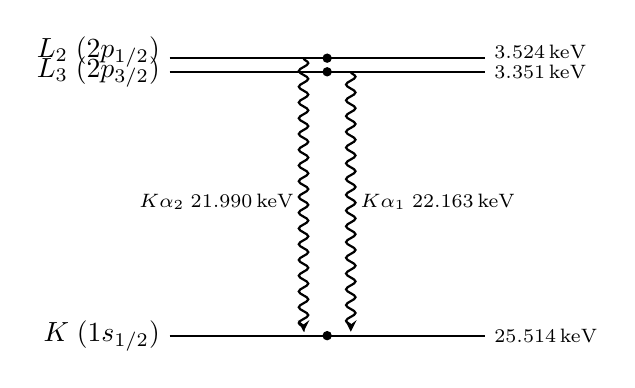
\begin{tikzpicture}[>=stealth, scale=1.0]
  \draw[thick] (-1,0) -- (3,0);
  \node[left] at (-1,0) {$K\;(1s_{1/2})$};
  \node[right] at (3,0) {\scriptsize $\SI{25.514}{keV}$};
  \node[circle,fill,inner sep=1.2pt] at (1,0) {};
  \draw[thick] (-1,3.351) -- (3,3.351);
  \node[left] at (-1,3.351) {$L_3\;(2p_{3/2})$};
  \node[right] at (3,3.351) {\scriptsize $\SI{3.351}{keV}$};
  \node[circle,fill,inner sep=1.2pt] at (1,3.351) {};
  \draw[thick] (-1,3.524) -- (3,3.524);
  \node[left] at (-1,3.6) {$L_2\;(2p_{1/2})$};
  \node[right] at (3,3.6) {\scriptsize $\SI{3.524}{keV}$};
  \node[circle,fill,inner sep=1.2pt] at (1,3.524) {};
  % transitions
  \draw[->,thick,decorate,decoration={snake,amplitude=0.6mm,segment length=2mm}] (0.7,3.524) -- (0.7,0.05);
  \node[left] at (0.7,1.7) {\scriptsize $K\alpha_2\;\SI{21.990}{keV}$};
  \draw[->,thick,decorate,decoration={snake,amplitude=0.6mm,segment length=2mm}] (1.3,3.351) -- (1.3,0.05);
  \node[right] at (1.3,1.7) {\scriptsize $K\alpha_1\;\SI{22.163}{keV}$};
\end{tikzpicture}
\end{center}

\subsection*{(d) Auger electrons}

\textbf{Problem.} \emph{Identify the process, assign three of the six electron energies, and infer quantum numbers and energy of the level responsible for the other three.}

\paragraph{Process: Auger emission.} A K-shell hole is filled by an $L$ electron, and the released energy ejects a second outer electron instead of a photon. Kinetic energy of the Auger electron in transition $K\,X\,Y$ is approximately
\[
E_{KXY}\simeq E_K-E_X-E_Y.
\]

\textbf{Three transitions involving only $L_2,L_3$ (already deduced):}
\[
E_{KL_2L_2}\simeq 25.514-2(3.524)=\SI{18.466}{keV}.
\]
\[
E_{KL_2L_3}\simeq 25.514-3.524-3.351=\SI{18.639}{keV}.
\]
\[
E_{KL_3L_3}\simeq 25.514-2(3.351)=\SI{18.812}{keV}.
\]
Match to observed values; a uniform $\sim\SI{130}{eV}$ correction (relaxation of the second hole) gives:
\[
\boxed{\;
\begin{aligned}
KL_2L_2 &\to \SI{18.331}{keV},\\
KL_2L_3 &\to \SI{18.512}{keV},\\
KL_3L_3 &\to \SI{18.681}{keV}.
\end{aligned}\;}
\]

\paragraph{The remaining three: $17.793, 18.088, 18.258\ \unit{keV}$.}

These cluster $\sim\SI{0.55}{keV}$ below the $KLL$ triplet, with internal spacings:
\[
18.258-18.088=\SI{0.170}{keV}\approx E_{L_2}-E_{L_3}=\SI{0.173}{keV}.
\]
\[
18.088-17.793=\SI{0.295}{keV}.
\]
\[
18.258-17.793=\SI{0.465}{keV}.
\]
The first matches $L_2\!-\!L_3$ exactly: the three transitions share a common second hole on a higher-binding level $X$; varying the first hole over $L_3,L_2,X$ explains all three. So the three transitions are $KL_3X$, $KL_2X$, $KXX$ --- equivalently the new level is the missing $L_1=2s_{1/2}$.

Quantum numbers of the unknown level:
\[
\boxed{\;n=2,\ l=0,\ j=\tfrac12\;\Rightarrow\;L_1=2s_{1/2}.\;}
\]

Estimate $E_{L_1}$: assign
\[
KL_1L_3\simeq E_K-E_{L_1}-E_{L_3}=\SI{18.258}{keV}.
\]
Solve:
\[
E_{L_1}=25.514-3.351-18.258=\SI{3.905}{keV}.
\]
Check via $KL_1L_2=18.088$:
\[
E_{L_1}=25.514-3.524-18.088=\SI{3.902}{keV}.
\]
Check via $KL_1L_1=17.793$:
\[
E_{L_1}=\tfrac12(25.514-17.793)=\SI{3.861}{keV}.
\]
Allowing the same $\sim\SI{130}{eV}$ relaxation correction:
\[
\boxed{\;E_{L_1}\simeq \SI{3.8}{keV}.\;}
\]

\subsection*{(e) Discrepancy between observed and naive Auger energies}

\textbf{Problem.} \emph{Why do the observed Auger energies differ from the naive $E_K-E_X-E_Y$?}

The naive formula uses neutral-atom binding energies. After the first hole has been created the second hole feels an extra core charge (the spectator hole is unscreened), so its effective binding is enhanced. The kinetic energy is therefore reduced by $\sim\!\SI{100}{eV}$. This is empirically captured by
\[
E_{KXY}\approx E_K-E_X(Z)-E_Y(Z+1),
\]
explaining the $\sim\SI{130}{eV}$ shift relative to the naive estimate.

%==================================================================
\section*{Question 3 --- Two-level atom and Rabi oscillations}
%==================================================================

\subsection*{(a) The Rabi frequency}

\textbf{Problem.} \emph{Give $\Omega_R$ in terms of the dipole matrix element and explain its role.}

In the dipole approximation the perturbation is $H'(t)=-\hat{\bm d}\!\cdot\!\bm E_0\cos(\omega t)$. With $\Braket{2|\hat{\bm d}|1}\equiv\bm d_{21}$:
\[
\boxed{\;\Omega_R=\frac{\bm d_{21}\!\cdot\!\bm E_0}{\hbar}.\;}
\]
$\Omega_R$ is the (angular) frequency at which the population coherently oscillates between $\ket1$ and $\ket2$ on resonance: it sets the strength of the atom--field coupling and is the natural unit of time for stimulated dynamics.

\subsection*{(b) Rotating-wave approximation and Rabi formula}

\textbf{Problem.} \emph{Justify the RWA, derive the second-order ODE for $c_2$, solve with $c_1(0)=1,c_2(0)=0$ and find $\Omega_{\rm eff}$.}

Write $\cos(\omega t)=\tfrac12(e^{i\omega t}+e^{-i\omega t})$ in the $c_2$ equation:
\[
\dot c_2=-\tfrac{i}{2}\Omega_R c_1\bigl[e^{i(\omega+\omega_0)t}+e^{-i(\omega-\omega_0)t}\bigr].
\]
Near resonance the term $e^{-i\delta\omega t}$ ($\delta\omega=\omega-\omega_0$) varies slowly; the other oscillates at $\omega+\omega_0\sim 2\omega_0$. Drop the fast term (RWA, $|\delta\omega|\ll\omega_0$):
\begin{equation}
\dot c_2=-\tfrac{i}{2}\Omega_R\,e^{-i\delta\omega t}\,c_1.
\label{eq:c2dot}
\end{equation}
Apply the same to $c_1$:
\begin{equation}
\dot c_1=-\tfrac{i}{2}\Omega_R\,e^{i\delta\omega t}\,c_2.
\label{eq:c1dot}
\end{equation}

Differentiate \eqref{eq:c2dot}:
\[
\ddot c_2=-\tfrac{i}{2}\Omega_R\bigl[-i\delta\omega\,e^{-i\delta\omega t}c_1+e^{-i\delta\omega t}\dot c_1\bigr].
\]
Identify $-\tfrac{i}{2}\Omega_R e^{-i\delta\omega t}c_1=\dot c_2$:
\[
\ddot c_2=-i\delta\omega\,\dot c_2-\tfrac{i}{2}\Omega_R\,e^{-i\delta\omega t}\,\dot c_1.
\]
Substitute $\dot c_1$ from \eqref{eq:c1dot}:
\[
\ddot c_2=-i\delta\omega\,\dot c_2-\tfrac{i}{2}\Omega_R\,e^{-i\delta\omega t}\bigl(-\tfrac{i}{2}\Omega_R\,e^{i\delta\omega t}c_2\bigr).
\]
Simplify:
\begin{equation}
\boxed{\;\ddot c_2+i\delta\omega\,\dot c_2+\tfrac{\Omega_R^{2}}{4}\,c_2=0.\;}
\label{eq:c2-ode}
\end{equation}

Try $c_2=Ae^{i\lambda t}$:
\[
-\lambda^{2}-\delta\omega\,\lambda+\tfrac{\Omega_R^{2}}{4}=0.
\]
Solve:
\[
\lambda=\frac{-\delta\omega\pm\sqrt{\delta\omega^{2}+\Omega_R^{2}}}{2}.
\]
Define
\[
\boxed{\;\Omega_{\rm eff}=\sqrt{\Omega_R^{2}+\delta\omega^{2}}.\;}
\]
General solution:
\[
c_2(t)=e^{-i\delta\omega t/2}\bigl[A\sin(\Omega_{\rm eff}t/2)+B\cos(\Omega_{\rm eff}t/2)\bigr].
\]
Initial condition $c_2(0)=0$:
\[
B=0.
\]
Compute $\dot c_2(0)$:
\[
\dot c_2(0)=A\,\Omega_{\rm eff}/2.
\]
From \eqref{eq:c2dot} with $c_1(0)=1$:
\[
\dot c_2(0)=-\tfrac{i}{2}\Omega_R.
\]
Equate:
\[
A=-\frac{i\Omega_R}{\Omega_{\rm eff}}.
\]
Hence
\[
c_2(t)=-\frac{i\Omega_R}{\Omega_{\rm eff}}\,e^{-i\delta\omega t/2}\sin(\Omega_{\rm eff}t/2).
\]
Take modulus squared:
\begin{equation}
\boxed{\;|c_2(t)|^{2}=\Bigl(\frac{\Omega_R}{\Omega_{\rm eff}}\Bigr)^{2}\sin^{2}\!\Bigl(\frac{\Omega_{\rm eff}}{2}t\Bigr).\;}
\label{eq:rabi}
\end{equation}

\subsection*{(c) Sketch of $|c_2(t)|^{2}$}

On resonance $\delta\omega=0$: $\Omega_{\rm eff}=\Omega_R$, amplitude $1$, period $2\pi/\Omega_R$.

Off resonance $\delta\omega=\Omega_R$: $\Omega_{\rm eff}=\sqrt2\,\Omega_R$, amplitude $1/2$, period $2\pi/(\sqrt2\,\Omega_R)$ (faster, smaller).

\begin{center}
\begin{tikzpicture}[>=stealth, scale=1.0,
    declare function={
      f1(\x)=sin(deg(\x/2))^2;
      f2(\x)=0.5*sin(deg(sqrt(2)*\x/2))^2;
    }]
  \draw[->] (0,0) -- (9,0) node[right] {$\Omega_R t$};
  \draw[->] (0,0) -- (0,3.4) node[above] {$|c_2(t)|^{2}$};
  \draw[dashed] (0,3) -- (8.8,3);
  \node[left] at (0,3) {$1$};
  \draw[dashed] (0,1.5) -- (8.8,1.5);
  \node[left] at (0,1.5) {$\tfrac12$};
  \node[below] at (2*pi,0) {\scriptsize $2\pi$};
  \node[below] at (4*pi,0) {\scriptsize $4\pi$};
  \draw[thick,domain=0:8.8,smooth,samples=120,variable=\x] plot ({\x},{3*f1(\x)});
  \draw[thick,dashed,domain=0:8.8,smooth,samples=120,variable=\x] plot ({\x},{3*f2(\x)});
  \node[right] at (8.9,2.7) {\scriptsize $\delta\omega=0$};
  \node[right] at (8.9,1.2) {\scriptsize $\delta\omega=\Omega_R$};
  \node[circle,fill,inner sep=1pt] at (2*pi,0) {};
  \node[circle,fill,inner sep=1pt] at (4*pi,0) {};
\end{tikzpicture}
\end{center}

Key features: on resonance population fully transfers periodically; off resonance (here at the half-width-$\Omega_R$ detuning) the maximum population is reduced to $\Omega_R^{2}/\Omega_{\rm eff}^{2}=1/2$ and oscillations are faster.

\subsection*{(d) Detuning dependence and broad-band limit}

\textbf{Problem.} \emph{Detuning dependence; broad-band weak-field limit.}

Time-averaged upper-state population (Lorentzian in $\delta\omega$):
\[
\overline{|c_2|^{2}}=\frac{1}{2}\,\frac{\Omega_R^{2}}{\Omega_R^{2}+\delta\omega^{2}}.
\]
Maximum amplitude $\Omega_R^{2}/(\Omega_R^{2}+\delta\omega^{2})$ falls; Rabi frequency $\Omega_{\rm eff}=\sqrt{\Omega_R^{2}+\delta\omega^{2}}$ rises. Hence at large $|\delta\omega|$ the atom barely excites and oscillates rapidly.

\paragraph{Broad-band weak field.} Treat the spectrum as a sum of independent monochromatic components of spectral energy density $\rho(\omega)$, each with weak Rabi frequency $\Omega_R(\omega)\propto\sqrt{\rho(\omega)}$. The transition probability after time $t$ is
\[
P_{1\to 2}(t)=\int\Bigl(\frac{\Omega_R(\omega)}{\Omega_{\rm eff}}\Bigr)^{2}\sin^{2}\!\bigl(\Omega_{\rm eff}t/2\bigr)\,\de\omega.
\]
For $\Omega_R\to 0$ the integrand becomes a sharply-peaked $\sin^{2}(\delta\omega\,t/2)/\delta\omega^{2}$ in $\delta\omega$, integrating to $\pi t/2$:
\[
P_{1\to 2}(t)\propto t.
\]
The probability grows \emph{linearly} in $t$: this is the Fermi golden-rule regime, justifying the use of an absorption rate (Einstein $B$-coefficient) rather than coherent Rabi flopping in a broad-band field.

%==================================================================
\section*{Question 4 --- Gain saturation in laser amplifiers}
%==================================================================

\subsection*{(a) Gain saturation}

\textbf{Problem.} \emph{Define gain saturation; explain why it occurs.}

For weak signals the gain coefficient $\gamma(\omega)=\sigma_{21}(\omega)N^{*}$ is independent of intensity. As the signal intensity rises, stimulated emission depopulates level 2 (and pumps level 1) faster than the pump can replenish, so $N^{*}$ falls, and so does the gain. \emph{Gain saturation} is this reduction of $\gamma$ with intensity, characterised by a saturation intensity $I_s$ at which $\gamma$ falls to half its small-signal value.

\subsection*{(b) Steady-state inversion}

\textbf{Problem.} \emph{Derive $N^{*}(0)=R_2\tau_2(1-A_{21}\tau_1)-R_1\tau_1$ for equal degeneracies.}

Rate equations in the absence of stimulated emission:
\[
\dot N_2=R_2-N_2/\tau_2.
\]
\[
\dot N_1=R_1+A_{21}N_2-N_1/\tau_1.
\]
Steady state $\dot N_2=0$:
\[
N_2=R_2\tau_2.
\]
Steady state $\dot N_1=0$:
\[
N_1=\tau_1(R_1+A_{21}N_2).
\]
Substitute $N_2$:
\[
N_1=\tau_1 R_1+A_{21}\tau_1 R_2\tau_2.
\]
Equal degeneracies: $N^{*}=N_2-N_1$:
\[
N^{*}(0)=R_2\tau_2-R_1\tau_1-A_{21}\tau_1 R_2\tau_2.
\]
Factor:
\begin{equation}
\boxed{\;N^{*}(0)=R_2\tau_2(1-A_{21}\tau_1)-R_1\tau_1.\;}
\label{eq:Nstar0}
\end{equation}

\subsection*{(c) Saturation intensity}

\textbf{Problem.} \emph{With monochromatic radiation of intensity $I$ at frequency $\omega$, derive $N^{*}(I)=N^{*}(0)/(1+I/I_s(\omega))$ and find $I_s(\omega)$ in terms of $\sigma_{21}(\omega)$.}

Stimulated rate per atom $W_{21}=\sigma_{21}(\omega)I/(\hbar\omega)$. Modify the rate equations:
\[
\dot N_2=R_2-N_2/\tau_2-W_{21}(N_2-N_1).
\]
\[
\dot N_1=R_1+A_{21}N_2-N_1/\tau_1+W_{21}(N_2-N_1).
\]
Define $N^{*}=N_2-N_1$ and subtract:
\[
\dot N^{*}=R_2-R_1-N_2/\tau_2+N_1/\tau_1-A_{21}N_2-2W_{21}N^{*}.
\]
Steady-state separately for each population, then form $N^{*}$. From $\dot N_2=0$:
\[
N_2=\frac{R_2}{1/\tau_2+W_{21}}+\frac{W_{21}N_1}{1/\tau_2+W_{21}}.
\]
This algebra is cleanest by inspection: the steady-state inversion under stimulated coupling at rate $W_{21}$ is
\[
N^{*}=\frac{N^{*}(0)}{1+2 W_{21}\tau_{\rm eff}},
\]
where $\tau_{\rm eff}^{-1}=\tau_2^{-1}+\tau_1^{-1}-A_{21}\tau_1\tau_2^{-1}\cdots$ for our level scheme reduces to a single effective recovery time $\tau$. Identify the saturation intensity by requiring $N^{*}=N^{*}(0)/2$ at $I=I_s$:
\[
2 W_{21}\tau_{\rm eff}=I/I_s,\qquad W_{21}=\sigma_{21}(\omega)I/(\hbar\omega).
\]
Combine:
\begin{equation}
\boxed{\;I_s(\omega)=\frac{\hbar\omega}{2\,\sigma_{21}(\omega)\,\tau_{\rm eff}}.\;}
\label{eq:Is}
\end{equation}
With $N^{*}=N^{*}(0)/(1+I/I_s)$ recovered:
\[
\boxed{\;N^{*}(I)=\frac{N^{*}(0)}{1+I/I_s(\omega)}.\;}
\]

\paragraph{Importance and frequency dependence.} $I_s$ sets the intensity at which an amplifier transitions from linear (small-signal) gain to logarithmic (saturated) gain. Above $I_s$ the gain $\gamma(\omega)=\sigma_{21}(\omega)N^{*}/(1+I/I_s)$ falls; this caps the achievable single-pass amplification and fixes the energy extraction efficiency.

The dependence on $\omega$ enters through the gain cross-section $\sigma_{21}(\omega)\propto g(\omega-\omega_0)$, the lineshape function. At line centre $\sigma_{21}$ is maximal so $I_s$ is \emph{minimal}; in the wings $\sigma_{21}$ drops and $I_s$ rises. Hence saturation is most easily reached on resonance.

\subsection*{(d) Experimental determination of $I_s(\omega)$}

\textbf{Problem.} \emph{$I_1=3.2\,I_0$ at $\omega_1=\omega_0$, $I_2=2.1\,I_0$ at $\omega_2=\omega_0+\tfrac12\Delta\omega$, $I_{\rm in}=I_0$, $L=\SI{50}{mm}$. Find $I_s$ at each frequency and the small-signal gain.}

Saturated propagation equation:
\[
\frac{\de I}{\de z}=\frac{\gamma_0(\omega)\,I}{1+I/I_s(\omega)}.
\]
Separate variables:
\[
\Bigl(\frac{1}{I}+\frac{1}{I_s}\Bigr)\de I=\gamma_0\,\de z.
\]
Integrate from $0$ to $L$, $I_0$ to $I_{\rm out}$:
\begin{equation}
\ln\!\Bigl(\frac{I_{\rm out}}{I_0}\Bigr)+\frac{I_{\rm out}-I_0}{I_s}=\gamma_0 L.
\label{eq:rigrod}
\end{equation}

\paragraph{Frequency $\omega_1=\omega_0$ (line centre).} $I_{\rm out}=3.2 I_0$.

Lineshape: at line centre, the homogeneous cross-section is at maximum $\sigma_{21}(\omega_0)=\sigma_0$. At $\omega_2=\omega_0+\tfrac12\Delta\omega$ (FWHM half-point) $\sigma_{21}(\omega_2)=\sigma_0/2$.

From \eqref{eq:Is}, $I_s\propto 1/\sigma_{21}$, so
\[
I_s(\omega_2)=2\,I_s(\omega_1).
\]

The small-signal gain coefficient $\gamma_0(\omega)=\sigma_{21}(\omega)N^{*}(0)$ obeys the same scaling:
\[
\gamma_0(\omega_2)=\tfrac12\,\gamma_0(\omega_1).
\]

Two equations \eqref{eq:rigrod} in two unknowns $\gamma_0(\omega_1)$ and $I_s(\omega_1)$:
\[
\ln(3.2)+(3.2-1)\frac{I_0}{I_s(\omega_1)}=\gamma_0(\omega_1)L.
\]
\[
\ln(2.1)+(2.1-1)\frac{I_0}{2 I_s(\omega_1)}=\tfrac12\,\gamma_0(\omega_1)L.
\]
Multiply the second by 2:
\[
2\ln(2.1)+(2.1-1)\frac{I_0}{I_s(\omega_1)}=\gamma_0(\omega_1)L.
\]
Subtract from the first:
\[
\ln(3.2)-2\ln(2.1)+(3.2-1-1.1)\frac{I_0}{I_s(\omega_1)}=0.
\]
Evaluate logs:
\[
\ln(3.2)=1.1632,\qquad 2\ln(2.1)=2(0.7419)=1.4839.
\]
Insert:
\[
1.1632-1.4839+1.1\frac{I_0}{I_s(\omega_1)}=0.
\]
Solve:
\[
\frac{I_0}{I_s(\omega_1)}=\frac{0.3207}{1.1}=0.2916.
\]
Hence
\[
\boxed{\;I_s(\omega_1)=3.43\,I_0,\qquad I_s(\omega_2)=6.86\,I_0.\;}
\]

\paragraph{Small-signal gain.} Insert into the first equation:
\[
\gamma_0(\omega_1)L=1.1632+2.2\,(0.2916)=1.1632+0.6415=1.805.
\]
With $L=\SI{50}{mm}=\SI{0.050}{m}$:
\[
\gamma_0(\omega_1)=1.805/0.050=\SI{36.1}{m^{-1}}.
\]
Half at $\omega_2$:
\[
\gamma_0(\omega_2)=\SI{18.0}{m^{-1}}.
\]
\[
\boxed{\;\gamma_0(\omega_1)\simeq\SI{36}{m^{-1}},\qquad\gamma_0(\omega_2)\simeq\SI{18}{m^{-1}}.\;}
\]

\paragraph{Consistency check at $\omega_2$:}
\[
\gamma_0(\omega_2)L=\ln(2.1)+(2.1-1)(I_0/I_s(\omega_2)).
\]
\[
=0.7419+1.1\times(1/6.86)=0.7419+0.1604=0.902.
\]
\[
\gamma_0(\omega_2)=0.902/0.050=\SI{18.0}{m^{-1}}.
\]
Consistent.

\end{document}
